\bta{磁场的综合应用}



\begin{enumerate}
\item
\exwhere{$ 2019 $ 年物理天津卷}
笔记本电脑机身和显示屏对应部位分别有磁体和霍尔元件。当显示屏开启
时磁体远离霍尔元件,电脑正常工作:当显示屏闭合时磁体靠近霍尔元件,屏幕熄灭,电脑进入休
眠状态。如图所示,一块宽为 $ a $、长为 $ c $ 的矩形半导体霍尔元件,元件内的导电粒子是电荷量为 $ e $ 的
自由电子,通入方向向右的电流时,电子的定向移动速度为 $ v $。当显示屏闭合时元件处于垂直于上
表面、方向向下的匀强磁场中,于是元件的前、后表面间出现电压 $ U $,以此控制屏幕的熄灭。则元
件的 \xzanswer{D} 
% TODO: \usepackage{graphicx} required
\begin{figure}[h!]
	\centering
	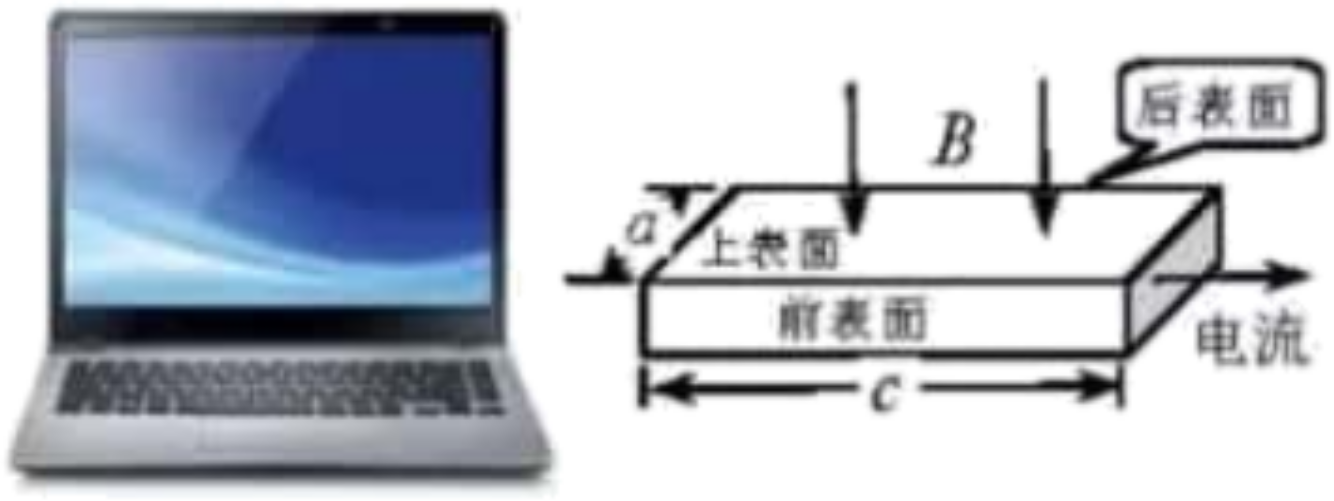
\includegraphics[width=0.4\linewidth]{picture/screenshot068}
\end{figure}


\fourchoices
{前表面的电势比后表面的低}
{前、后表面间的电压 $ U $ 与 $ v $ 无关}
{前、后表面间的电压 $ U $ 与 $ c $ 成正比}
{自由电子受到的洛伦兹力大小为$\frac{e U}{a}$}


\item 
\exwhere{$ 2014 $ 年物理江苏卷}
如图所示,导电物质为电子的霍尔元件位于两串联线圈之间,线圈中电流为 $ I $,线圈间产生匀
强磁场,磁感应强度大小 $ B $ 与 $ I $ 成正比,方向垂直于霍尔元件的两侧面,此时通过霍尔元件的电
流为 $ I_{H} $,与其前后表面相连的电压表测出的霍尔电压 $ U_{H} $ 满足: $U_{H}=k \frac{I_{H} B}{d}$,式中 $ k $ 为霍尔系
数,$ d $ 为霍尔元件两侧面间的距离,电阻 $ R $ 远大于 $ R_{L} $,
霍尔元件的电阻可以忽略,则 \xzanswer{CD} 
\begin{figure}[h!]
	\centering
	\includesvg[width=0.33\linewidth]{picture/svg/GZ-3-tiyou-1268}
\end{figure}


\fourchoices
{霍尔元件前表面的电势低于后表面}
{若电源的正负极对调,电压表将反偏}
{$ I_{H} $ 与 $ I $ 成正比}
{电压表的示数与 $ R_{L} $ 消耗的电功率成正比}




\item 
\exwhere{$ 2018 $年浙江卷($ 4 $月选考)}
压力波测量仪可将待测压力波转换为电压信号,
其原理如图$ 1 $所示。压力波$ p $($ t $)进入弹性盒后,通过与铰链$ O $相连的“$ -| $”型轻杆$ L $,驱动杆端头$ A $处
的微型霍尔片在磁场中沿$ x $轴方向做微小振动,其位移$ x $与压力$ p $成正比($ x= \alpha p $,$ \alpha >0 $)。霍尔片的放
大图如图$ 2 $所示,它由长$ \times $宽$ \times $厚$ =a \times b \times d $、单位体积内自由电子数为$ n $的$ N $型半导体制成。磁场方向垂
直于$ x $轴向上,磁感应强度大小为$ B=B_{0} $($ 1- \beta |x| $),$ \beta >0 $。无压力波输入时,霍尔片静止在$ x=0 $处,此
时给霍尔片通以沿$ C_{1} C_{2} $方向的电流$ I $,则在侧面上$ D_{1} $、$ D_{2} $两点间产生霍尔电压$ U_{0} $。
\begin{enumerate}
	%\renewcommand{\labelenumi}{\arabic{enumi}.}
	% A(\Alph) a(\alph) I(\Roman) i(\roman) 1(\arabic)
	%设定全局标号series=example	%引用全局变量resume=example
	%[topsep=-0.3em,parsep=-0.3em,itemsep=-0.3em,partopsep=-0.3em]
	%可使用leftmargin调整列表环境左边的空白长度 [leftmargin=0em]
	\item
指出$ D_{1} $、$ D_{2} $两点哪点电势高;


\item 
推导出$ U_{0} $与$ I $、$ B_{0} $之间的关系式(提示:电流$ I $与自由电子定向移动速率$ v $之间关系为$ I=nevbd $,
其中$ e $为电子电荷量);

\item 
弹性盒中输入压力波$ p $($ t $),霍尔片中通以相同电流,测得霍尔电压$ U_{H} $随时间$ t $变化图像如图$ 3 $。
忽略霍尔片在磁场中运动产生的电动势和阻尼,求压力波的振幅和频率。(结果用$ U_{0} $、$ U_{1} $、$ t_{0} $、$ \alpha $
及$ \beta $表示)

\end{enumerate}
\begin{figure}[h!]
	\centering
\begin{subfigure}{0.4\linewidth}
	\centering
	\includesvg[width=0.7\linewidth]{picture/svg/GZ-3-tiyou-1266} 
	\caption{}\label{}
\end{subfigure}
\begin{subfigure}{0.4\linewidth}
	\centering
	\includesvg[width=0.7\linewidth]{picture/svg/GZ-3-tiyou-1267} 
	\caption{}\label{}
\end{subfigure}
\end{figure}


\banswer{
	\begin{enumerate}
		%\renewcommand{\labelenumi}{\arabic{enumi}.}
		% A(\Alph) a(\alph) I(\Roman) i(\roman) 1(\arabic)
		%设定全局标号series=example	%引用全局变量resume=example
		%[topsep=-0.3em,parsep=-0.3em,itemsep=-0.3em,partopsep=-0.3em]
		%可使用leftmargin调整列表环境左边的空白长度 [leftmargin=0em]
		\item
		$ D_{1} $ 点电势高
		\item 
		电子受力平衡:$ e vB_{0}=eE_{H} $ 得到$U_{0}=E_{H} b=\frac{1}{n e} \frac{I B_{0}}{d}$
		\item 
		霍尔电压 $U_{H}(t)=U_{0}(1-\alpha \beta|p|)$,
		振幅: $A=\frac{1}{\alpha \beta}\left(1-\frac{U_{1}}{U_{0}}\right)$,
		频率: $f=\frac{1}{2 t_{0}}$
	\end{enumerate}
}



\item 
\exwhere{$ 2014 $ 年理综福建卷}
如图,某一新型发电装置的发电管是横截面为矩形的水平管道,管道的长为 $ L $、宽度为 $ d $、高
为 $ h $,上下两面是绝缘板,前后两侧面 $ M $、$ N $ 是电阻可忽略的导体板,两导体板与开关 $ S $ 和定值电
阻 $ R $ 相连。整个管道置于磁感应强度大小为 $ B $,方向沿 $ z $ 轴正方向的匀强磁场中。管道内始终充满
电阻率为$ \rho $的导电液体(有大量的正、负离子),且开关闭合前后,液体在管道进、出口两端压强差
的作用下,均以恒定速率 $ v_{0} $ 沿 $ x $ 轴正向流动,液体所受的摩擦阻力不变。
\begin{enumerate}
	%\renewcommand{\labelenumi}{\arabic{enumi}.}
	% A(\Alph) a(\alph) I(\Roman) i(\roman) 1(\arabic)
	%设定全局标号series=example	%引用全局变量resume=example
	%[topsep=-0.3em,parsep=-0.3em,itemsep=-0.3em,partopsep=-0.3em]
	%可使用leftmargin调整列表环境左边的空白长度 [leftmargin=0em]
	\item
求开关闭合前,$ M $、$ N $ 两板间的电势差大小 $ U_{0} $;


\item 
求开关闭合前后,管道两端压强差的变化$ \Delta p $;

\item 
调整矩形管道的宽和高,但保持其它量和矩形
管道的横截面 $ S=dh $ 不变,求电阻 $ R $ 可获得的最大功
率 $ P_{m} $ 及相应的宽高比 $ d/h $ 的值。

	
\end{enumerate}
\begin{figure}[h!]
	\flushright
	\includesvg[width=0.25\linewidth]{picture/svg/GZ-3-tiyou-1269}
\end{figure}


\banswer{
	\begin{enumerate}
		%\renewcommand{\labelenumi}{\arabic{enumi}.}
		% A(\Alph) a(\alph) I(\Roman) i(\roman) 1(\arabic)
		%设定全局标号series=example	%引用全局变量resume=example
		%[topsep=-0.3em,parsep=-0.3em,itemsep=-0.3em,partopsep=-0.3em]
		%可使用leftmargin调整列表环境左边的空白长度 [leftmargin=0em]
		\item
		$U_{0}=B d v_{0}$
		\item 
		$\Delta p=\frac{L d v_{0} B^{2}}{L h R+d \rho}$
		\item 
		$P=\left(\frac{B L v_{0}}{\frac{L R}{d}+\frac{\rho}{h}}\right)^{2} R$\\
		当 $\frac{d}{h}=\frac{L R}{\rho}$ 时, 电阻 $R$ 获得的最大功率 $P_{m}=\frac{L S v_{0}^{2} B^{2}}{4 \rho}$
	\end{enumerate}
}


\item 
\exwhere{$ 2013 $ 年浙江卷}
为了降低潜艇噪音,提高其前进速度,可用电磁推进器替代螺旋桨。潜艇下方有左、
右两组推进器,每组由 $ 6 $ 个相同的、用绝缘材料制成的直线通道推进器构成,其原理示意图如下。
在直线通道内充满电阻率$ \rho =0.2 \ \Omega \cdot m $ 的海水,通道中 $ a \times b \times c=0.3 \ m \times 0.4 \ m \times 0.3 \ m $ 的空间内,存在由超导
线圈产生的匀强磁场,其磁感应强度 $ B=6.4 \ T $、方向垂直通道侧面向外。磁场区域上、下方各有
$ a \times b=0.3 \ m \times 0.4 \ m $ 的金属板 $ M $、$ N $,当其与推进器专用直流电源相连后,在两板之间的海水中产生了
从 $ N $ 到 $ M $,大小恒为 $ I=1.0 \times 10^{3} \ A $ 的电流,设电流只存在于磁场区域。不计电源内阻及导线电阻,
海水密度$ \rho _{m}=1.0 \times 10^{3} \ kg/m^{3} $。
\begin{enumerate}
	%\renewcommand{\labelenumi}{\arabic{enumi}.}
	% A(\Alph) a(\alph) I(\Roman) i(\roman) 1(\arabic)
	%设定全局标号series=example	%引用全局变量resume=example
	%[topsep=-0.3em,parsep=-0.3em,itemsep=-0.3em,partopsep=-0.3em]
	%可使用leftmargin调整列表环境左边的空白长度 [leftmargin=0em]
	\item
求一个直线通道推进器内磁场对通电海水的作用力大小,并判断其方向;

\item 
在不改变潜艇结构的前提下,简述潜艇如何转弯?如何“倒车”?

\item 
当潜艇以恒定速度 $ v_{0} =30 \ m /s $ 前进时,海水在出口处相对于推进器的速度 $ v=34 \ m /s $,思考专用
直流电源所提供的电功率如何分配,求出相应功率的大小。

	
\end{enumerate}
\begin{figure}[h!]
	\centering
	\includesvg[width=0.73\linewidth]{picture/svg/GZ-3-tiyou-1270}
\end{figure}



\banswer{
	\begin{enumerate}
		%\renewcommand{\labelenumi}{\arabic{enumi}.}
		% A(\Alph) a(\alph) I(\Roman) i(\roman) 1(\arabic)
		%设定全局标号series=example	%引用全局变量resume=example
		%[topsep=-0.3em,parsep=-0.3em,itemsep=-0.3em,partopsep=-0.3em]
		%可使用leftmargin调整列表环境左边的空白长度 [leftmargin=0em]
		\item
		$ 1.92 \times 10^{3} \ N $,方向向右
		\item 
		开启或关闭不同个数的左、右两侧的直线通道推进器,实施转弯。
		改变电流方向,或改变磁场方向,可以改变海水所受磁场力的方向,实施“倒车”。
		\item 
		电源提供的电功率中的第一部分为牵引功率,$ P_{1} =F _{ \text{牵} } v_{0} =6.9 \times 10^{5} \ W $\\
		电源提供的电功率中的第二部分为单位时间内海水的焦耳热功率,
		推进器内海水的电阻 $R=\rho \frac{L}{S}=\frac{\rho c}{a b} =0.5 \ \Omega $,
		$ P_{2} =12 I^{2} R=6 \times 10^{6} \ W $\\
		电源提供的电功率中的第三部分为单位时间内海水动能的增加量\\
		单位时间内通过推进器的水的质量为$m=\rho_{m} b c v_{\text {水对地 }}=480 \ kg$\\
		单位时间内其动能增加为$P_{3}=12 \cdot \frac{1}{2} m v_{\text {水对地 }}^{2}=4.6 \times 10^{4} \ W$
	\end{enumerate}
}

\item 
\exwhere{$ 2012 $ 年理综天津卷}
对铀 $ 235 $ 的进一步研究在核能的开发和利用中具有重要的意义。如图所示,质量为 $ m $、
电荷量为 $ q $ 的铀 $ 235 $ 离子,从容器 $ A $ 下方的小孔 $ S_{1} $ 不断飘入加速电场,其初速度可视为零,然后
经过小孔 $ S_{2} $ 垂直与磁场方向进入磁感应强度为 $ B $ 的均强磁场中,做半径为 $ R $ 的匀速圆周运动,离
子行进半个圆周后离开磁场并被收集,离开磁场时离子束的等效电流 $ I $。不考虑离子重力及离子间
的相互作用。
\begin{enumerate}
	%\renewcommand{\labelenumi}{\arabic{enumi}.}
	% A(\Alph) a(\alph) I(\Roman) i(\roman) 1(\arabic)
	%设定全局标号series=example	%引用全局变量resume=example
	%[topsep=-0.3em,parsep=-0.3em,itemsep=-0.3em,partopsep=-0.3em]
	%可使用leftmargin调整列表环境左边的空白长度 [leftmargin=0em]
	\item
求加速电场的电压 $ U $;

\item 
求出在离子被收集的过程中任意时间 $ t $ 内收集到离子的质
量 $ M $;


\item 
实际上加速电压的大小在 $ U \pm \Delta U $ 范围内微小变化。若容
器 $ A $ 中有电荷量相同的铀 $ 235 $ 和铀 $ 238 $ 两种离子,如前述情况
它们经电场加速后进入磁场中发生分离,为使这两种离子在磁
场中运动的轨迹不发生交叠,
$\frac{\Delta U}{U}$
应小于多少?(结果用百分
数表示,保留两位有效数字)

	

\end{enumerate}
\begin{figure}[h!]
	\flushright
	\includesvg[width=0.25\linewidth]{picture/svg/GZ-3-tiyou-1271}
\end{figure}



\banswer{
	\begin{enumerate}
		%\renewcommand{\labelenumi}{\arabic{enumi}.}
		% A(\Alph) a(\alph) I(\Roman) i(\roman) 1(\arabic)
		%设定全局标号series=example	%引用全局变量resume=example
		%[topsep=-0.3em,parsep=-0.3em,itemsep=-0.3em,partopsep=-0.3em]
		%可使用leftmargin调整列表环境左边的空白长度 [leftmargin=0em]
		\item
		$U=\frac{q B^{2} R^{2}}{2 m}$
		\item 
		$M=\frac{m I t}{q}$
		\item 
		$\frac{\Delta U}{U}<\frac{m^{\prime}-m}{m^{\prime}+m}=\frac{238 u-235 u}{238 u+235 u}=\frac{3}{473}=0.63 \%$
	\end{enumerate}
}




\item
\exwhere{$ 2011 $ 年理综北京卷}
利用电场和磁场,可以将比荷不同的离子分开,这种方法在化学分析和原子核技术等
领域有重要的应用。
如图所示的矩形区域 $ ACDG $($ AC $ 边足够长)中存在垂直于纸面的匀强磁场,$ A $ 处有一狭缝。离子
源产生的离子,经静电场加速后穿过狭缝沿垂直于 $ GA $ 边且垂于磁场的方向射入磁场,运动到 $ GA $
边,被相应的收集器收集,整个装置内部为真空。
已知被加速的两种正离子的质量分别是 $ m_{1} $ 和 $ m_{2} $
$ ( m_{1} > m_{2} ) $,电荷量均为 $ q $。加速电场的电势差为 $ U $,
离子进入电场时的初速度可以忽略,不计重力,也不
考虑离子间的相互作用。
\begin{enumerate}
	%\renewcommand{\labelenumi}{\arabic{enumi}.}
	% A(\Alph) a(\alph) I(\Roman) i(\roman) 1(\arabic)
	%设定全局标号series=example	%引用全局变量resume=example
	%[topsep=-0.3em,parsep=-0.3em,itemsep=-0.3em,partopsep=-0.3em]
	%可使用leftmargin调整列表环境左边的空白长度 [leftmargin=0em]
	\item
求质量为 $ m_{1} $ 的离子进入磁场时的速率 $ v_{1} $;



\item 
当感应强度的大小为 $ B $ 时,求两种离子在 $ G_{A} $ 边
落点的间距 $ s $;

\item 
在前面的讨论中忽略了狭缝宽度的影响,实际装置中狭缝具有一定宽度。若狭缝过宽,可能
使两束离子在 $ GA $ 边上的落点区域交叠,导致两种离子无法完全分离。
设磁感应强度大小可调,$ GA $ 边长为定值 $ L $,狭缝宽度为 $ d $,狭缝右边缘在 $ A $ 处;离子可以从狭
缝各处射入磁场,入射方向仍垂直于 $ GA $ 边且垂直于磁场。为保证上述两种离子能落在 $ GA $ 边上并
被完全分离,求狭缝的最大宽度。
	

\end{enumerate}
\begin{figure}[h!]
	\flushright
	\includesvg[width=0.25\linewidth]{picture/svg/GZ-3-tiyou-1272}
\end{figure}


\banswer{
	\begin{enumerate}
		%\renewcommand{\labelenumi}{\arabic{enumi}.}
		% A(\Alph) a(\alph) I(\Roman) i(\roman) 1(\arabic)
		%设定全局标号series=example	%引用全局变量resume=example
		%[topsep=-0.3em,parsep=-0.3em,itemsep=-0.3em,partopsep=-0.3em]
		%可使用leftmargin调整列表环境左边的空白长度 [leftmargin=0em]
		\item
		$v_{1}=\sqrt{\frac{2 q U}{m_{1}}}$
		\item 
		$s=2 R_{1}-2 R_{2}=\sqrt{\frac{8 U}{q B^{2}}}\left(\sqrt{m_{1}}-\sqrt{m_{2}}\right)$
		\item 
		$d_{m}=\frac{\sqrt{m_{1}}-\sqrt{m_{2}}}{2 \sqrt{m_{1}}-\sqrt{m_{2}}}$
	\end{enumerate}
}




\item 
\exwhere{$ 2011 $ 年理综天津卷}
回旋加速器在核科学、核技术、核医学等高新技术领域得到了广泛应用,有力地推动
了现代科学技术的发展。
\begin{enumerate}
	%\renewcommand{\labelenumi}{\arabic{enumi}.}
	% A(\Alph) a(\alph) I(\Roman) i(\roman) 1(\arabic)
	%设定全局标号series=example	%引用全局变量resume=example
	%[topsep=-0.3em,parsep=-0.3em,itemsep=-0.3em,partopsep=-0.3em]
	%可使用leftmargin调整列表环境左边的空白长度 [leftmargin=0em]
	\item
当今医学影像诊断设备 $ PET/CT $ 堪称“现代医学高科
技之冠”,它在医疗诊断中,常利用能放射正电子的同位
素碳 $ 11 $ 作示踪原子。碳 $ 11 $ 是由小型回旋加速器输出的高
速质子轰击氮 $ 14 $ 获得,同时还产生另一粒子,试写出核
反应方程。若碳 $ 11 $ 的半衰期$ \tau $为 $ 20 \ min $,经 $ 2.0 \ h $ 剩余碳
$ 11 $的质量占原来的百分之几?(结果取 $ 2 $ 位有效数字)


\item 
回旋加速器的原理如图,$ D_{1} $ 和 $ D_{2} $ 是两个中空的半径为 $ R $ 的半圆金属盒,它们接在电压一定、
频率为 $ f $ 的交流电源上,位于 $ D_{1} $ 圆心处的质子源 $ A $ 能不断产生质子(初速度可以忽略,重力不计),
它们在两盒之间被电场加速,$ D_{1} $、$ D_{2} $ 置于与盒面垂直的磁感应强度为 $ B $ 的匀强磁场中。若质子束
从回旋加速器输出时的平均功率为 $ P $,求输出时质子束的等效电流 $ I $ 与 $ P $、$ B $、$ R $、$ f $ 的关系式(忽略
质子在电场中的运动时间,其最大速度远小于光速)。

\item 
试推理说明:质子在回旋加速器中运动时,随轨道半径 $ r $ 的增大,同一盒中相邻轨道的半径
之差$ \Delta r $ 是增大、减小还是不变?

	
\end{enumerate}
\begin{figure}[h!]
	\flushright
	\includesvg[width=0.25\linewidth]{picture/svg/GZ-3-tiyou-1273}
\end{figure}


\banswer{
	\begin{enumerate}
		%\renewcommand{\labelenumi}{\arabic{enumi}.}
		% A(\Alph) a(\alph) I(\Roman) i(\roman) 1(\arabic)
		%设定全局标号series=example	%引用全局变量resume=example
		%[topsep=-0.3em,parsep=-0.3em,itemsep=-0.3em,partopsep=-0.3em]
		%可使用leftmargin调整列表环境左边的空白长度 [leftmargin=0em]
		\item
		核反应方程为 ${ }_{7}^{14} \mathrm{~N}+{ }_{1}^{1} \mathrm{H} \rightarrow{ }_{6}^{1} \mathrm{C}+{ }_{2}^{4} \mathrm{He}$\\
		$\frac{m_{t}}{m_{0}}=\left(\frac{1}{2}\right)^{\frac{t}{\tau}}=\left(\frac{1}{2}\right)^{\frac{120}{20}}=1.6 \%$
		\item 
		$I=\frac{P}{\pi B R^{2} f}$
		\item 
		设 $ k $($ k \in N \star $)为同一盒子中质子运动轨道半径的序数,相邻的轨道半径分别为 $ r_k $,$ r_{k+1} $($ r_k>r_{k+1} $),
		$\Delta r_{k}=r_{k+1}-r_{k}$,在相应轨道上质子对应的速度大小分别为 $ v_k $,$ v_{k+1} $,$ D_{1} $、$ D_{2} $ 之间的电压为 $ U $。\\
		令 $C=\frac{4 m U}{q B^{2}}$,得 $\Delta r_{k}=\frac{C}{r_{k}+r_{k+1}}$。
		相邻轨道半径 $r_{k+1}, r_{k+2}$ 之差 $\Delta r_{k+1}=r_{k+2}-r_{k+1}$,同理 $\quad \Delta r_{k}=\frac{C}{r_{k+1}+r_{k+2}}$。\\
		天为 $r_{k+2}>r_{k}, \quad$ 比较 $\Delta r_{k},  \Delta r_{k+1}$ 得 $\Delta r_{k+1}<\Delta r_{k}$,说明随轨道半径$ r $的增大,同一盒中相邻轨道的半径之差$\Delta r$减小。\\
		(方法不止一种)	
	\end{enumerate}
}


\item 
\exwhere{$ 2014 $ 年理综天津卷}
同步加速器在粒子物理研究中有重要的应用,其基本原理简化为如图所示的模型.$ M $、
$ N $ 为两块中心开有小孔的平行金属板.质量为 $ m $、电荷量为$ +q $ 的粒子
$ A $(不计重力)从 $ M $ 板小孔飘入板间,初速度可视为零.每当 $ A $ 进入
板间,两板的电势差变为 $ U $,粒子得到加速,当 $ A $ 离开 $ N $ 板时,两板
的电荷量均立即变为零.两板外部存在垂直纸面向里的匀强磁场,$ A $
在磁场作用下做半径为 $ R $ 的圆周运动,$ R $ 远大于板间距离.$ A $ 经电场
多次加速,动能不断增大,为使 $ R $ 保持不变,磁场必须相应地变化.不计粒子加速时间及其做圆周
运动产生的电磁辐射,不考虑磁场变化对粒子速度的影响及相对论效应.求
\begin{enumerate}
	%\renewcommand{\labelenumi}{\arabic{enumi}.}
	% A(\Alph) a(\alph) I(\Roman) i(\roman) 1(\arabic)
	%设定全局标号series=example	%引用全局变量resume=example
	%[topsep=-0.3em,parsep=-0.3em,itemsep=-0.3em,partopsep=-0.3em]
	%可使用leftmargin调整列表环境左边的空白长度 [leftmargin=0em]
	\item
$ A $ 运动第 $ 1 $ 周时磁场的磁感应强度 $ B_{1} $ 的大小;

\item 
在 $ A $ 运动第 $ n $ 周的时间内电场力做功的平均功率 $ \bar{P}_{n} $;

\item 
若有一个质量也为 $ m $、电荷量为$ +kq $($ k $ 为大于 $ 1 $ 的整数)的粒子 $ B $(不计重力)与 $ A $ 同时从
$ M $ 板小孔飘入板间,$ A $、$ B $ 初速度均可视为零,不计两者间的相互作用,除此之外,其他条件均不
变.下图中虚线、实线分别表示 $ A $、$ B $ 的运动轨迹.在 $ B $ 的轨迹半径远大于板间距离的前提下,请
指出哪个图能定性地反映 $ A $、$ B $ 的运动轨迹,并经推导说明理由.

	
\end{enumerate}
\pfourchoices
{\includesvg[width=3cm]{picture/svg/GZ-3-tiyou-1274}}
{\includesvg[width=3cm]{picture/svg/GZ-3-tiyou-1275}}
{\includesvg[width=3cm]{picture/svg/GZ-3-tiyou-1276}}
{\includesvg[width=3cm]{picture/svg/GZ-3-tiyou-1277}}
\begin{figure}[h!]
	\flushright
	\includesvg[width=0.25\linewidth]{picture/svg/GZ-3-tiyou-1278}
\end{figure}




\banswer{
	\begin{enumerate}
		%\renewcommand{\labelenumi}{\arabic{enumi}.}
		% A(\Alph) a(\alph) I(\Roman) i(\roman) 1(\arabic)
		%设定全局标号series=example	%引用全局变量resume=example
		%[topsep=-0.3em,parsep=-0.3em,itemsep=-0.3em,partopsep=-0.3em]
		%可使用leftmargin调整列表环境左边的空白长度 [leftmargin=0em]
		\item
		$B_{1}=\frac{1}{R} \sqrt{\frac{2 m U}{q}}$
		\item 
		$B_{1}=\frac{1}{R} \sqrt{\frac{2 m U}{q}}$
		\item 
		A
		 \quad 
		理由略 
	\end{enumerate}
}


\item 
\exwhere{$ 2015 $ 年理综浙江卷}
使用回旋加速器的实验需要把离子束从加速器中引出,离子束引
出的方法有磁屏蔽通道法和静电偏转法等。质量为 $ m $,速度为 $ v $ 的离子在回旋加速器内旋转,旋转
轨道是半径为 $ r $ 的圆,圆心在 $ O $ 点,轨道在垂直纸面向外的匀强磁场中,磁感应强度为 $ B $。

为引出离子束,使用磁屏蔽通道法设计引出器。引出器原理如图所示,一对圆弧形金属板组成
弧形引出通道,通道的圆心位于 $ O ^{\prime} $点($ O ^{\prime} $点图中未
画出)。引出离子时,令引出通道内磁场的磁感应强
度降低,从而使离子从 $ P $ 点进入通道,沿通道中心
线从 $ Q $ 点射出。已知 $ OQ $ 长度为 $ L $。$ OQ $ 与 $ OP $ 的夹
角为$ \theta $。
\begin{enumerate}
	%\renewcommand{\labelenumi}{\arabic{enumi}.}
	% A(\Alph) a(\alph) I(\Roman) i(\roman) 1(\arabic)
	%设定全局标号series=example	%引用全局变量resume=example
	%[topsep=-0.3em,parsep=-0.3em,itemsep=-0.3em,partopsep=-0.3em]
	%可使用leftmargin调整列表环境左边的空白长度 [leftmargin=0em]
	\item
求离子的电荷量 $ q $ 并判断其正负;



\item 
离子从 $ P $ 点进入,$ Q $ 点射出,通道内匀强磁场的磁感应强度应降为 $ B ^{\prime} $,求 $ B ^{\prime} $;

\item 
换用静电偏转法引出离子束,维持通道内的原有磁感应强度 $ B $ 不变,在内外金属板间加直流
电压,两板间产生径向电场,忽略边缘效应。为使离子仍从 $ P $ 点进入,$ Q $ 点射出,求通道内引出轨
迹处电场强度 $ E $ 的方向和大小。

\end{enumerate}
\begin{figure}[h!]
	\flushright
	\includesvg[width=0.25\linewidth]{picture/svg/GZ-3-tiyou-1279}
\end{figure}


\banswer{
	\begin{enumerate}
		%\renewcommand{\labelenumi}{\arabic{enumi}.}
		% A(\Alph) a(\alph) I(\Roman) i(\roman) 1(\arabic)
		%设定全局标号series=example	%引用全局变量resume=example
		%[topsep=-0.3em,parsep=-0.3em,itemsep=-0.3em,partopsep=-0.3em]
		%可使用leftmargin调整列表环境左边的空白长度 [leftmargin=0em]
		\item
		$q=\frac{m v}{B r}$,正电荷
		\item 
		$ B ^{\prime} = \frac{m v(2 r-2 L \cos \theta)}{q\left(r^{2}+L^{2}-2 r R \cos \theta\right)} $
		\item 
		电场强度的方向沿径向向外\\
		$E=B v-\frac{m v^{2}(2 r-2 L \cos \theta)}{q\left(r^{2}+L^{2}-2 r R \cos \theta\right)}$
	\end{enumerate}
}


\item 
\exwhere{$ 2016 $ 年新课标  \lmd{1}  卷}
现代质谱仪可用来分析比质子重很多倍的离子,其示意图如图所示,其中
加速电压恒定。质子在入口处从静止开始被加速电场加速,
经匀强磁场偏转后从出口离开磁场。若某种一价正离子在入
口处从静止开始被同一加速电场加速,为使它经匀强磁场偏
转后仍从同一出口离开磁场,需将磁感应强度增加到原来的
$ 12 $倍。此离子和质子的质量比约为 \xzanswer{D} 
\begin{figure}[h!]
	\centering
	\includesvg[width=0.23\linewidth]{picture/svg/GZ-3-tiyou-1280}
\end{figure}

\fourchoices
{$ 11 $}
{$ 12 $}
{$ 121 $}
{$ 144 $}



\item 
\exwhere{$ 2016 $ 年浙江卷}
为了进一步提高回旋加速器的能量,科学家建造了“扇形聚焦回旋加
速器”。在扇形聚焦过程中,离子能以不变的速率在闭合平衡轨道上周期性旋转。

扇形聚焦磁场分布的简化图如图所示,圆心为 $ O $ 的圆形区域等分成六个扇形区域,其中三个为峰区,
三个为谷区,峰区和谷区相间分布。峰区内存在方向垂直纸面向里的匀强磁场,磁感应强度为 $ B $,
谷区内没有磁场。质量为 $ m $,电荷量为 $ q $ 的正离子,以不变的速率 $ v $ 旋转,其闭合平衡轨道如图中
虚线所示。
\begin{enumerate}
	%\renewcommand{\labelenumi}{\arabic{enumi}.}
	% A(\Alph) a(\alph) I(\Roman) i(\roman) 1(\arabic)
	%设定全局标号series=example	%引用全局变量resume=example
	%[topsep=-0.3em,parsep=-0.3em,itemsep=-0.3em,partopsep=-0.3em]
	%可使用leftmargin调整列表环境左边的空白长度 [leftmargin=0em]
	\item
求闭合平衡轨道在峰区内圆弧的半径 $ r $,并判断离子旋转的方向是顺时针还是逆时针;

\item 
求轨道在一个峰区内圆弧的圆心角$ \theta $,及离子绕闭合平
衡轨道旋转的周期 $ T $;

\item 
在谷区也施加垂直纸面向里的匀强磁场,磁感应
强度为 $ B ^{\prime} $,新的闭合平衡轨道在一个峰区内的圆心角$ \theta $
变为 $ 90 \degree $,求 $ B ^{\prime} $和 $ B $ 的关系。已知:$\sin (\alpha \pm \beta)=\sin \alpha \cos \beta \pm \cos \alpha \sin \beta, \quad \cos \alpha=1-2 \sin ^{2} \frac{\alpha}{2}$。
	
\end{enumerate}
\begin{figure}[h!]
	\flushright
	\includesvg[width=0.25\linewidth]{picture/svg/GZ-3-tiyou-1281}
\end{figure}


\banswer{
	\begin{enumerate}
		%\renewcommand{\labelenumi}{\arabic{enumi}.}
		% A(\Alph) a(\alph) I(\Roman) i(\roman) 1(\arabic)
		%设定全局标号series=example	%引用全局变量resume=example
		%[topsep=-0.3em,parsep=-0.3em,itemsep=-0.3em,partopsep=-0.3em]
		%可使用leftmargin调整列表环境左边的空白长度 [leftmargin=0em]
		\item
		$r=\frac{m v}{B q} $; 旋转方向为逆时针方向
		\item 
		$\theta=\frac{2 \pi}{3} \quad T=\frac{(2 \pi+3 \sqrt{3}) m}{q B}$
		\item 
		$B^{\prime}=\frac{\sqrt{3}-1}{2} B$
	\end{enumerate}
}



\item 
\exwhere{$ 2017 $ 年江苏卷}
一台质谱仪的工作原理如图所示。大量的甲、乙两种离子飘入电压为
$ U_{0} $ 的加速电场,其初速度几乎为 $ 0 $,经过加速后,通过宽为 $ L $ 的狭缝 $ MN $ 沿着与磁场垂直的方向进
入磁感应强度为 $ B $ 的匀强磁场中,最后打到照相底片上。已
知甲、乙两种离子的电荷量均为$ +q $,质量分别为 $ 2m $ 和 $ m $,
图中虚线为经过狭缝左、右边界 $ M $、$ N $ 的甲种离子的运动轨
迹,不考虑离子间的相互作用.
\begin{enumerate}
	%\renewcommand{\labelenumi}{\arabic{enumi}.}
	% A(\Alph) a(\alph) I(\Roman) i(\roman) 1(\arabic)
	%设定全局标号series=example	%引用全局变量resume=example
	%[topsep=-0.3em,parsep=-0.3em,itemsep=-0.3em,partopsep=-0.3em]
	%可使用leftmargin调整列表环境左边的空白长度 [leftmargin=0em]
	\item
求甲种离子打在底片上的位置到 $ N $ 点的最小距离 $ x $;

\item 
在答题卡的图中用斜线标出磁场中甲种离子经过的区
域,并求该区域最窄处的宽度 $ d $;

\item 
若考虑加速电压有波动,在$\left(U_{0}-\Delta U\right)$到$\left(U_{0}+\Delta U\right)$之间变化,要使甲、乙两种离子在
底片上没有重叠,求狭缝宽度 $ L $ 满足的条件.

	
\end{enumerate}
\begin{figure}[h!]
	\flushright
	\includesvg[width=0.25\linewidth]{picture/svg/GZ-3-tiyou-1282}
\end{figure}

\banswer{
	\begin{enumerate}
		%\renewcommand{\labelenumi}{\arabic{enumi}.}
		% A(\Alph) a(\alph) I(\Roman) i(\roman) 1(\arabic)
		%设定全局标号series=example	%引用全局变量resume=example
		%[topsep=-0.3em,parsep=-0.3em,itemsep=-0.3em,partopsep=-0.3em]
		%可使用leftmargin调整列表环境左边的空白长度 [leftmargin=0em]
		\item
		$x=\frac{4}{B} \sqrt{\frac{m U_{0}}{q}}-L$
		\item 
		$d=\frac{2}{B} \sqrt{\frac{m U_{0}}{q}}-\sqrt{\frac{4 m U_{0}}{q B^{2}}-\frac{L^{2}}{4}}$
		\item 
		$L<\frac{2}{B} \sqrt{\frac{m}{q}}\left[2 \sqrt{\left(U_{0}-\Delta U\right)}-\sqrt{2\left(U_{0}+\Delta U\right)}\right]$
	\end{enumerate}
}








\end{enumerate}

